\documentclass[a4paper,10pt,ngerman]{scrartcl}
\usepackage{babel}
\usepackage[T1]{fontenc}
\usepackage[utf8x]{inputenc}
\usepackage[a4paper,margin=2.5cm,footskip=0.5cm]{geometry}

% Die nächsten drei Felder bitte anpassen:
\newcommand{\Aufgabe}{Aufgabe 1: Transformers} % Aufgabennummer und Aufgabennamen angeben
\newcommand{\TeilnahmeId}{79418}                  % Teilnahme-ID angeben
\newcommand{\Name}{Fabian Schwarz}             % Name des Bearbeiter / der Bearbeiterin dieser Aufgabe angeben


% Kopf- und Fußzeilen
\usepackage{scrlayer-scrpage, lastpage}
\setkomafont{pageheadfoot}{\large\textrm}
\lohead{\Aufgabe}
\cohead{\Name}
\rohead{Teilnahme-ID: \TeilnahmeId}
\cfoot*{\thepage{}/\pageref{LastPage}}

% Position des Titels
\usepackage{titling}
\setlength{\droptitle}{-1.0cm}

% Für mathematische Befehle und Symbole
\usepackage{amsmath}
\usepackage{amssymb}

\usepackage{float}
% Für Bilder
\usepackage{graphicx}

% Für Algorithmen
\usepackage{algpseudocode}

% Für Quelltext
\usepackage{listings, listings-rust}
\usepackage{color}
\definecolor{mygreen}{rgb}{0,0.6,0}
\definecolor{mygray}{rgb}{0.5,0.5,0.5}
\definecolor{mymauve}{rgb}{0.58,0,0.82}
\lstset{
    keywordstyle=\color{blue},commentstyle=\color{mygreen},
    stringstyle=\color{mymauve},rulecolor=\color{black},
    basicstyle=\footnotesize\ttfamily,numberstyle=\tiny\color{mygray},
    captionpos=b, % sets the caption-position to bottom
    keepspaces=true, % keeps spaces in text
    numbers=left, numbersep=5pt, showspaces=false,showstringspaces=true,
    showtabs=false, stepnumber=2, tabsize=2, title=\lstname
}
\lstdefinelanguage{JavaScript}{ % JavaScript ist als einzige Sprache noch nicht vordefiniert
    keywords={break, case, catch, continue, debugger, default, delete, do, else, finally, for, function, if, in, instanceof, new, return, switch, this, throw, try, typeof, var, void, while, with},
    morecomment=[l]{//},
    morecomment=[s]{/*}{*/},
    morestring=[b]',
    morestring=[b]",
    sensitive=true
}

% Diese beiden Pakete müssen zuletzt geladen werden
\usepackage{amsopn}
\usepackage{amstext}
\usepackage{hyperref}
\usepackage{cleveref}
\usepackage{subcaption}

% Daten für die Titelseite
\title{\textbf{\Huge\Aufgabe}}
\author{\LARGE Teilnahme-ID: \LARGE \TeilnahmeId \\\\
\LARGE Bearbeiter/-in dieser Aufgabe: \\
\LARGE \Name\\\\}
\date{\LARGE\today}

\lstdefinestyle{plain}{
    language={},
    keywordstyle=\color{black},
    commentstyle=\color{black},
    stringstyle=\color{black},
    numbers=none,
    italicconsole=false
}

\lstset{frame=tb,
    language=Rust,
    aboveskip=3mm,
    belowskip=1mm,
    showstringspaces=false,
    columns=flexible,
    basicstyle={\small\ttfamily},
    numbers=none,
    numberstyle=\tiny\color{gray},
    keywordstyle=\color{blue},
    commentstyle=\color{dkgreen},
    stringstyle=\color{mauve},
    breaklines=true,
    breakatwhitespace=true,
    tabsize=3
}

\begin{document}

    \maketitle
    \tableofcontents

    \vspace{0.5cm}


    \section{Lösungsidee}
    Man modelliert jede Figur als einen ungerichteten, zusammenhängenden Graphen $G = (V, E)$. Die Knotenmenge $V$
    besteht hier aus den Steckplättchen, und die Kantenmenge $E$ aus den Stiften. Jeder Stift $e \in E$ ist hier aus
    einer Achse (horizontal bzw. vertikal) und einer Richtung (-1 bzw. +1) zusammengesetzt.

    Man bemerkt, dass Stifte, die Teil eines Zyklus sind, nicht gedreht werden können, da die Figur sonst ``zerreißt''.
    Man kondensiert den Graphen also zu einem neuen Graphen $G'$, in dem alle Knoten, die durch Zyklen verbunden sind,
    zu einem Superknoten (S) zusammengefasst sind. Dies sieht beispielsweise so aus:

    \begin{figure}[H]
        \centering
        \begin{subfigure}[b]{0.2\textwidth}
            \centering
            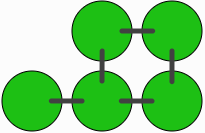
\includegraphics[width=\textwidth]{figur}
            \caption{Die Figur}
            \label{fig:step1}
        \end{subfigure}%
        \hfill
        \begin{subfigure}[b]{0.2\textwidth}
            \centering
            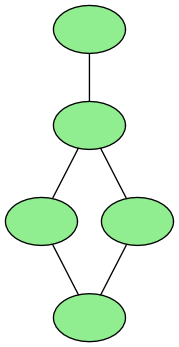
\includegraphics[width=\textwidth]{figur_graph}
            \caption{Der resultierende, zyklische Graph}
            \label{fig:step2}
        \end{subfigure}%
        \hfill
        \begin{subfigure}[b]{0.2\textwidth}
            \centering
            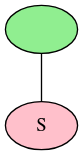
\includegraphics[width=\textwidth]{figur_superblock}
            \caption{Der kondensierte Graph}
            \label{fig:step3}
        \end{subfigure}
        \label{fig:figure0}
    \end{figure}

    Schließlich markiert man die Stifte mit ihren entsprechenden Richtungen:

    \begin{figure}[H]
        \centering
        \begin{minipage}{0.1\textwidth}
            \centering
            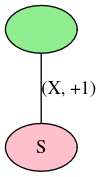
\includegraphics[width=\textwidth]{figur_labeled}
        \end{minipage}
        \hfill
        \begin{minipage}{0.85\textwidth}
            Der Stift ist horizontal, daher $X$, und verläuft von dem Ursprungsknoten aus nach rechts, daher $+1$.
            Man stellt hier fest, dass nach Beseitigung aller Zyklen der Graph, da er ja bereits zusammenhängend ist,
            einen Baum darstellt.
        \end{minipage}\label{fig:figure}
    \end{figure}

    Der Ursprungsknoten muss arbiträr, aber eindeutig, ausgewählt werden. Man hat aktuell noch keinerlei Wissen darüber,
    welcher Knoten welchem Gegenknoten im anderen Graphen entspricht. Es macht daher Sinn, die Zentren des Baums zu
    verwenden, wie sich in der Umsetzung zeigt.
    Ein komplexeres Beispiel könnte wie folgt aussehen:

    \begin{figure}[H]
        \centering
        \begin{subfigure}[b]{0.3\textwidth}
            \centering
            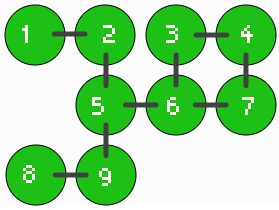
\includegraphics[width=\textwidth]{figur2}
            \caption{Die Figur}
            \label{fig:1step1}
        \end{subfigure}%
        \hfill
        \begin{subfigure}[b]{0.2\textwidth}
            \centering
            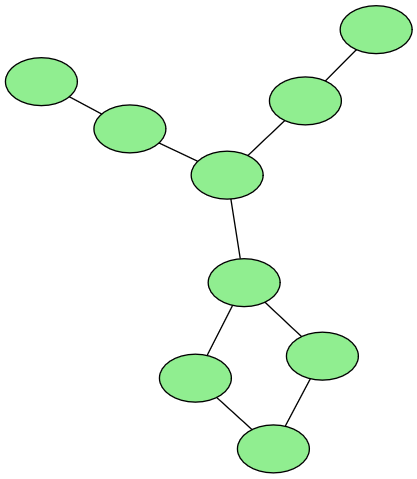
\includegraphics[width=\textwidth]{figur2_graph}
            \caption{Der resultierende, zyklische Graph}
            \label{fig:1step2}
        \end{subfigure}%
        \hfill
        \begin{subfigure}[b]{0.2\textwidth}
            \centering
            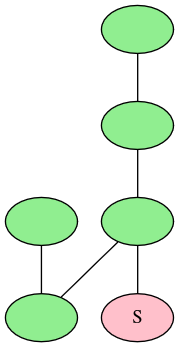
\includegraphics[width=\textwidth]{figur2_superblock}
            \caption{Der kondensierte Graph}
            \label{fig:1step3}
        \end{subfigure}
        \begin{subfigure}[b]{0.2\textwidth}
            \centering
            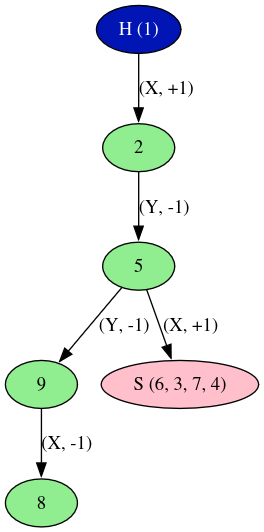
\includegraphics[width=\textwidth]{figur2_labeled}
            \caption{Der Graph mit Richtungsangaben}
            \label{fig:1step4}
        \end{subfigure}
        \label{fig:figure1}
    \end{figure}

    Zu Beginn werden den Plättchen beliebige Indices verliehen. Diese bleiben bei der Umwandlung in den Graphen
    natürlich erhalten, sind nur hier nicht abgebildet. Es werden erneut Zyklen zu Superblöcken kondensiert, und
    schließlich ein hier noch arbiträrer Ursprungsknoten (H) gewählt, von welchem aus der Graph traversiert und die
    Verbindungen beschriftet werden. Der Graph bleibt ungerichtet, ist hier aber, um das Traversieren zu kennzeichnen,
    mit Pfeilen dargestellt. Im Superknoten ist gespeichert, aus welchen Knoten dieser zusammengesetzt ist.

    Bei einer 180°-Drehung um einen Stift beobachtet man, dass alle Stifte parallel zur Drehachse ihre Richtung
    behalten, während alle senkrechten Stifte das Vorzeichen ihrer Richtung ändern. Ein Beispiel:

    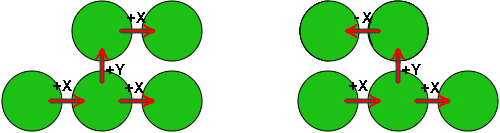
\includegraphics{figur3}

    Hier wird um den ``+Y''-Stift gedreht.

    Aus diesen Bedingungen lassen sich also Regeln für die Überführbarkeit zweier Figuren in einander anhand ihrer
    kondensierten Bäume bestimmen:
    \begin{itemize}
        \item Die Bäume A und B müssen isomorph sein, das heißt, die gleiche Anzahl an Knoten und Kanten haben, sowie
        Kanten auf den gleichen Achsen zwischen entsprechenden Knoten. Besteht der eine Baum also ausgehend von seiner
        Wurzel aus $V_1 = (+X, +Y, -X)$, so muss $V_2$ auch eine $(\pm X, \pm Y, \pm X)$ Abfolge sein.
        \item Zyklen müssen in beiden Figuren identisch sein, d.h., die gleiche Länge und die gleiche Abfolge von
        X- und Y-Verbindungen besitzen; die genaue Richtung ($\pm1$) ist erstmal irrelevant.
        \item In Baum B muss es pro Drehung genau ein Plättchen $P$ geben, dass als Drehpunkt fungiert. An ihm ist eine
        Drehachse $X$ oder $Y$ definiert. Alle Stifte, die über diese Drehachse an $P$ hängen, behalten ihre Richtung
        bei. Alle Stifte, die über die andere Achse an $P$ hängen, folgen den oben festgestellten Regeln: laufen sie
        parallel zur Drehachse, behalten sie ihre Richtung identisch bei; andernfalls ändert sich das Vorzeichen der
        Richtung.
        \item Zyklen müssen entweder vollständig identisch bleiben, d.h., identische Abfolgen an Verbindungen besitzen,
        oder, wenn sie gedreht wurden, nach der oben genannten Inversionsregel übereinstimmen. Beispielsweise kann
        $(+Y, +X, -Y, -X)$ nur identisch bleiben, zu $(-Y, +X, +Y, -X)$ oder zu $(+Y, -X, -Y, +X)$ werden. Diese
        Abfolgen haben natürlich keinen festen Startpunkt, d.h. $(+Y, +X, -Y, -X) = (-X, +Y, +X, -Y)$.
    \end{itemize}

    Gesondert sind Figuren zu betrachten, in welchen zwei Stifte gleichzeitig gedreht werden müssen, um die Figuren in
    einander zu überführen, da dies eine unzulässige Transformation ist. Jeder Zwischenschritt der Überführung, d.h. an
    einem einzelnen Plättchen und Stift, muss eine gültige Gitterkonfiguration darstellen. Wenn ein Zyklus in
    der Zielfigur so orientiert ist, dass sie nur durch eine gleichzeitige Drehung an zwei parallelen Stiften oder
    durch ein Überlappen mit schon vorhandenen Plättchen entstehen kann, wird die Figur als nicht überführbar eingestuft.

    \section{Umsetzung}
    Zu Beginn werden die Figuren eingelesen und als ungerichtete, gewichtete Graphen dargestellt. Die Gewichte sind hier
    die Richtung, bestehen also aus \texttt{axis} $\in {X, Y}$ und \texttt{sign} $\in {-1, +1}$.

    Um nun Zyklen zu erkennen, werden die Graphen mithilfe einer Tiefensuche in zweifach zusammenhängende Komponenten
    (\textit{Biconnected Components} nach Hopcroft and Tarjan (1973)\footnote{
        Hopcroft, J., \& Tarjan, R. (1973). Algorithm 447: efficient algorithms for graph manipulation.
        \textit{Communications of the ACM}, \textit{16}(6), 372–378. https://doi.org/10.1145/362248.362272
    }) geteilt. Artikulationspunkte sind mögliche Drehpunkte unserer Figur, die resultierenden ``Blöcke'' die starren
    Zyklen. Hierfür werden während der DFS alle Kanten auf einen Stack gelegt und, sobald ein Artikulationspunkt
    gefunden wird, alle Plättchen bis zu diesem Punkt als starrer Block betrachtet.

    Ein Artikulationspunkt ermittelt sich wie folgt:
    \begin{enumerate}
        \item Man traversiere den Graphen wie gewöhnlich in einer DFS, wobei alle traversierten Kanten auf einen Stack
        gelegt werden.
        \item Jedem Knoten wird eine Entdeckungszeit (en.\ \textit{discovery time}) \texttt{disc} zugewiesen, die für
        jeden Ablaufschritt inkrementiert wird. Ein zweites Feld \texttt{low} wird ebenfalls auf die Entdeckungszeit
        gesetzt.
        \item Während jeder Backtracking-Phase betrachte man:
        \begin{enumerate}
            \item für jeden Knoten $u$, rückwärts gehend, all seine (bereits besuchten) Nachbarn $v_i$, bis auf seinen
            direkten Vorgänger. Die von allen Nachbarn $v_i$ geringste \texttt{disc} übernimmt der Knoten $u$
            als \texttt{low}.
            \item für jede Kante $u \to v$, rückwärts gehend\footnote{Im forward-pass wurde also eine Kante $u \to v$
                abgelaufen; eigentlich läuft man hier von $v \to u$ rückwärts, dennoch wird die Kante hier als
                $u \to v$ beschrieben, wobei $u$ die ``ältere'' ist.},
            ob $v.\texttt{low} \geq u.\texttt{disc}$. Falls eine Gleichheit vorliegt, handelt es sich um einen
            Artikulationspunkt. Alle Knoten, die seit Beginn des backward-pass abgelaufen wurden, werden in den
            Artikulationspunkt als Superknoten vereint.\footnote{Der Artikulationspunkt ist der Punkt, der den Block mit
            dem Rest des Graphen verbindet. Die Wurzel der DFS ist nur dann ein Artikulationspunkt, wenn sie im
            DFS-Baum mehr als ein Kind hat.}
            Wenn der \texttt{low}-Wert echt größer ist, ist diese
            Verbindung eine Brücke, d.h.\ ein drehbarer Stift, und wird im resultierenden Baum zu einer Kante zwischen
            zwei (Super-)Knoten.
        \end{enumerate}
    \end{enumerate}

    Hiermit zerfällt die Figur in eine Menge von Superknoten, Artikulationspunkten (gewöhnlichen Plättchen) und Brücken,
    die sich zu dem kondensierten Baum zusammenfassen lassen (dem sog. \textit{block-cut tree}).
    Ein solcher Baum behält nun also folgende Informationen:
    \begin{itemize}
        \item Jeder Superknoten beinhält seine interne, zyklische Abfolge an Verbindungen, z.B. $(+X, +Y, -X, -Y)$,
        sowie seine Verbindungen nach außen
        \item Jedes Plättchen, das kein Teil eines Zyklus ist, bleibt ein Knoten
        \item Die Brücken, also alle Kanten außerhalb von Zyklen, werden zu den Kanten des Baums
    \end{itemize}

    Nun erfolgen die ersten Überprüfungen:
    \begin{enumerate}
        \item Haben beide Bäume die gleiche Anzahl an Knoten und Kanten?
        \item Sind die (ungeordneten) Listen der Grad-Zahlen der Knoten identisch?
    \end{enumerate}
    Ist eine der Überprüfungen falsch, sind die Figuren nicht in einander überführbar.

    Um nun zwei Bäume zu vergleichen, müssen sie in eine Form gebracht werden, in der die genaue Indizierung der Knoten
    für Vergleiche irrelevant wird. Hierzu werden von beiden Bäumen sukzessiv alle Blätter entfernt, bis nur noch 1
    oder 2 Knoten übrig bleiben. Diese Punkte werden Zentren genannt, die folgend als Wurzeln der Bäume verwendet
    werden. Hat einer der Bäume zwei Zentren, der andere jedoch nur eines, können die Bäume nicht isomorph sein.
    Haben beide Bäume zwei Zentren, wird das erste Zentrum von Baum $A$ mit beiden Zentren des Baums $B$ Gegengeprüft,
    und damit folgende Schritte zwei mal durchgeführt. Nur wenn beide scheitert, scheitert die ganze Überprüfung.

    Von den Wurzeln $R_A$ und $R_B$ aus wird nun der Baum traversiert, und eine Signatur erstellt. Diese setzt sich aus
    einer beliebig, aber immer gleich, sortierten Liste der Signaturen der Kinder und Achsen zu ihnen zusammen.
    Ein Beispiel:

    \begin{figure}[H]
        \centering
        \begin{minipage}{0.25\textwidth}
            \centering
            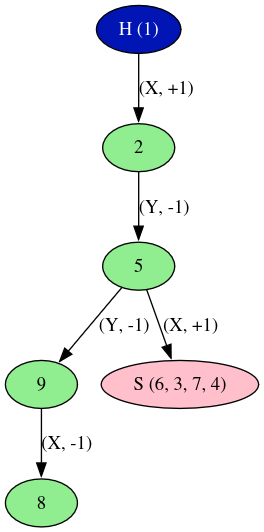
\includegraphics[width=\textwidth]{figur2_labeled}
        \end{minipage}
        \hfill
        \begin{minipage}{0.7\textwidth}
            Hier ermittelt sich Knoten $5$ als Zentrum. Also wird der Baum, entgegen der in der Lösungsidee gewählten
            Richtung, von ihm aus traversiert: Er hat die Kinder $2$, $9$, und $S(6, 3, 7, 4)$. Es wird  sich für eine
            Sortierung nach Index entschieden, also ergibt sich (vorerst) die Signatur: \texttt{[(+Y, 2), (-Y, 9),
            (+X, S(...))]}. Die Knoten werden nun erneut nach ihren Signaturen aufgelöst. Knoten 2 hat Knoten 1 als
            Kind, der ein Blatt ist. Knoten 9 hat 8 als Kind, ebenfalls ein Blatt. Der Superknoten $S$ hat intern seine
            Abfolge von Steckachsen gespeichert, also wird diese als seine Signatur eingefügt. Daher erweitert sich die
            Signatur insgesamt zu \texttt{[(+Y, [(-X, "Blatt")]), (-Y, [(-X, "Blatt")]),(+X, [S(+Y, +X, -Y, -X);])]}.
            Die gewählte Signatur von S ist hier beispielhaft ein einfacher Zyklus aus 4 Knoten; die Vorzeichen
            entsprechen nicht genau dem Beispiel von oben. Nach dem Semikolon würde wie gewohnt eine Liste der
            Nachbarknoten des Superknotens folgen, wenn er welche hätte. Diese Sonderregel ist wichtig, da sonst später
            die Übereinstimmung der Zyklen nicht geprüft werden kann. Es ist zu beachten, dass die Achsenabfolgen
            innerhalb von Superknoten zyklisch sind, d.h.\ weiterhin $(+Y, +X, -Y, -X) = (-X, +Y, +X, -Y)$, und so
            weiter. Auch Zyklen, die die Abfolge genau ``rückwärts'' haben, sind identisch.
        \end{minipage}\label{fig:figure2}
    \end{figure}

    Wenn die Signaturen zweier Bäume nun übereinstimmen, sind sie garantiert isomorph. Hierbei dürfen die Vorzeichen
    der Verbindungen abweichen, da sich diese durch Drehungen ja ändern können; es wird nur auf gleiches Vorkommen
    von $X$ und $Y$ geachtet. Stimmen die Signaturen nicht überein, sind sie nicht in einander überführbar.

    Nun wird sich parallel in beiden Bäumen von den Blättern bis zur Wurzel hochgearbeitet:
    \begin{itemize}
        \item Blätter sind immer von Baum $A$ zu Baum $B$ überführbar.
        \item Für jeden inneren Knoten wird geprüft, dass die Vorzeichen seiner Signatur zwischen den zwei Bäumen
        entweder exakt identisch, für alle $X$ umgekehrt, für alle $Y$ umgekehrt, oder für alle Verbindungen
        umgekehrt sind. Diese Vorzeichenregeln gelten auch innerhalb von Superknoten.
    \end{itemize}
    Ein Beispiel:

    Baum A hat die Signatur

    \texttt{[(+Y, [(-X, "Blatt")]), (-Y, [(-X, "Blatt")]),(+X, [S(+Y, +X, -Y, -X);])]}.

    Baum B hat die Signatur

    \texttt{[(+Y, [(+X, "Blatt")]), (-Y, [(-X, "Blatt")]),(+X, [S(-Y, +X, +Y, -X);])]}.

    Die Signaturen sind in ihren Abfolgen der Achsen $X$ und $Y$ identisch. Der erste Knoten \texttt{[(-X, "Blatt")]}
    wurde um die $Y$-Achse gedreht, wodurch sich das Vorzeichen von $X$ geändert hat. Der Zyklus $S$ wurde um die
    $X$-Achse gedreht, wodurch sich die Vorzeichen aller internen $Y$-Verbindungen geändert haben. (Im Code ist das
    anders umgesetzt, da Hashes effizienter sind als String Manipulation oder Listenoperationen.)

    Wenn auch diese Überprüfung gelingt, bedeutet dies, dass die Figuren in einander überführbar sind.
    Diese Überprüfung allein würde für die Lösung des Problems genügen, jedoch können durch die vorherigen Überprüfungen
    einige trivialen Negativbeispiele früh erkannt werden.

    Die interne Struktur der Superblöcke wird durch eine Liste von Richtungsvektoren $(\Delta x, \Delta y)$
    repräsentiert. Beim rekursiven Vergleich wird sichergestellt, dass bei einer angenommenen Drehung um eine Achse
    nicht nur die Brücken-Stifte im Baum, sondern auch alle internen Vektoren des Blocks konsistent transformiert werden.
    Durch die Verwendung der Baumzentren als Wurzeln und den anschließenden Abgleich aller möglichen Drehungen
    ($X$, $Y$, beide oder keine) pro Gelenk wird sichergestellt, dass nur physisch konsistente Transformationen zu
    einem positiven Ergebnis führen.

    \section{Laufzeit}\label{sec:laufzeit}
    Für $V$ Plättchen mit $E$ Verbindungen ist die Erstellung des Block-Cut-Trees über DFS $O(V + E)$. Die Suche
    der Zentren ist annähernd $O(V)$. Das Generieren der Signaturen ist aufgrund der Sortierung der Listen mit je
    maximal 4 Elementen unter $O(V \cdot \log(4))$ \footnote{
        \url{https://doc.rust-lang.org/std/primitive.slice.html#method.sort_by_key}
    } und damit $O(V)$.
    Der Lösungsansatz ist also auch für größere $V$ und $E$ effizient.

    \section{Werkzeuge}
    Der Code wurde vollständig in Rust 1.94.1 (e408947bf 2026-03-25) geschrieben.
    Das \href{https://crates.io/crates/petgraph}{\texttt{petgraph} Crate}
    wurde für eine optimierte Implementierung von Graphen verwendet. Es verwaltet die Lifetimes von Knoten und Kanten
    intern, was einigen Boilerplate-Code erspart.

    \section{Beispiele}

    \begin{lstlisting}[style=plain]
        1
        2
        3
    \end{lstlisting}


    \section{Quellcode}
    Auslassungen sind hier mit \texttt{/* [...] */} markiert.

    \begin{lstlisting}[style=colouredRust, label={lst:maincode}]
        fn solve() {
            return;
        }
    \end{lstlisting}

\end{document}
